\section{lemma11}
\begin{lemma}
\end{lemma}

Suppose we have a Riemann Sphere $C$ and a diagram $(C,\iota,\xi)$ and a regular cell complex refinement $\overline{(C,\iota,\xi)}$ and a sheaf $\mathfrak{F}$ singular supported on it such that when restricted to a small disk $D\subset C$ the refinement is as the following figure where two dimensional strata are labeled by tuples and numbers:

\begin{figure}[H] % Optional: [h] means here, [t] for top, [b] for bottom, [p] for page of floats
    \centering
    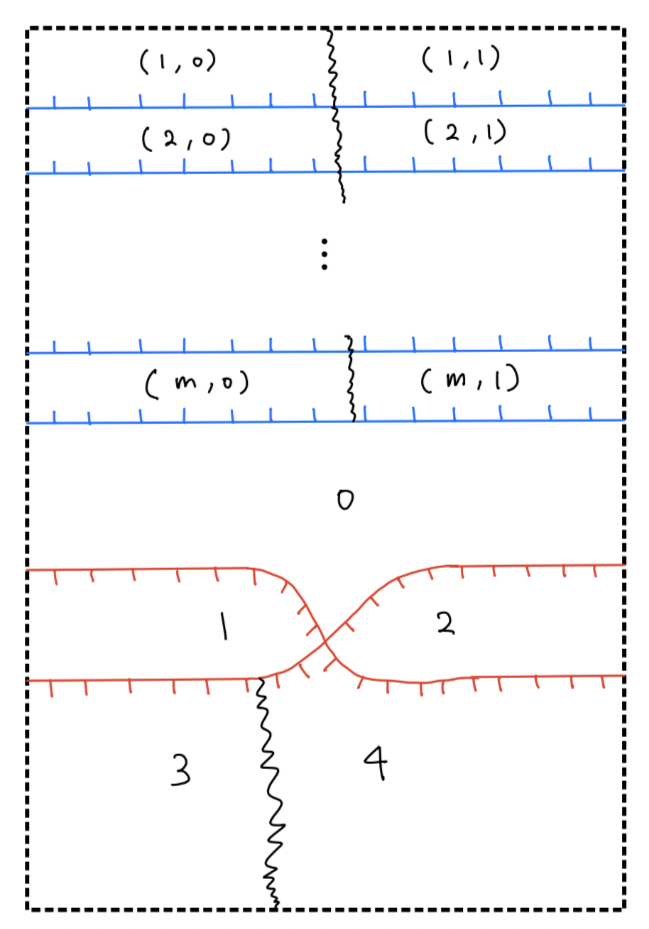
\includegraphics[scale=0.95]{diagrams/lemma11/1.png} % Adjust the width as needed
    \caption{Your caption here}
    \label{fig:your-label}
\end{figure}

Stalks:\\
- $(i,0),(i,1)$: $\mathbb{m+1-i}$\\
- 0 : $0$\\
- 1,2 : $\mathbb{C}$\\
- 3,4 : $\mathbb{C}^2$\\

Generization maps :\\

- $(i,0)\rightarrow (i,1)$ : $\mathbb{C}^{m-i+1}\rightarrow\mathbb{C}^{m-i+1}$, $D_{i,m}$\\
- 1$\rightarrow$4 : $\mathbb{C}\rightarrow\mathbb{C}^2$ where $e_1\mapsto (a,b)^T$\\
- 3$\rightarrow$4 : $\mathbb{C}^2 \rightarrow \mathbb{C}^2$ where $e_1\mapsto (a,b)^T$ and $e_2\mapsto (0,d)^T$\\
- all the other maps crossing the red strands are $\iota_f$\\
- all the other maps crossing the blue strands are $\iota_l$\\
- rest of the maps are zero maps\\

Now we will define isotopy starting from the above sheaf $\mathfrak{F}$ inductively on the number of blue strands so that the final sheaf $\mathfrak{F}'$ is
\begin{figure}[H] % Optional: [h] means here, [t] for top, [b] for bottom, [p] for page of floats
    \centering
    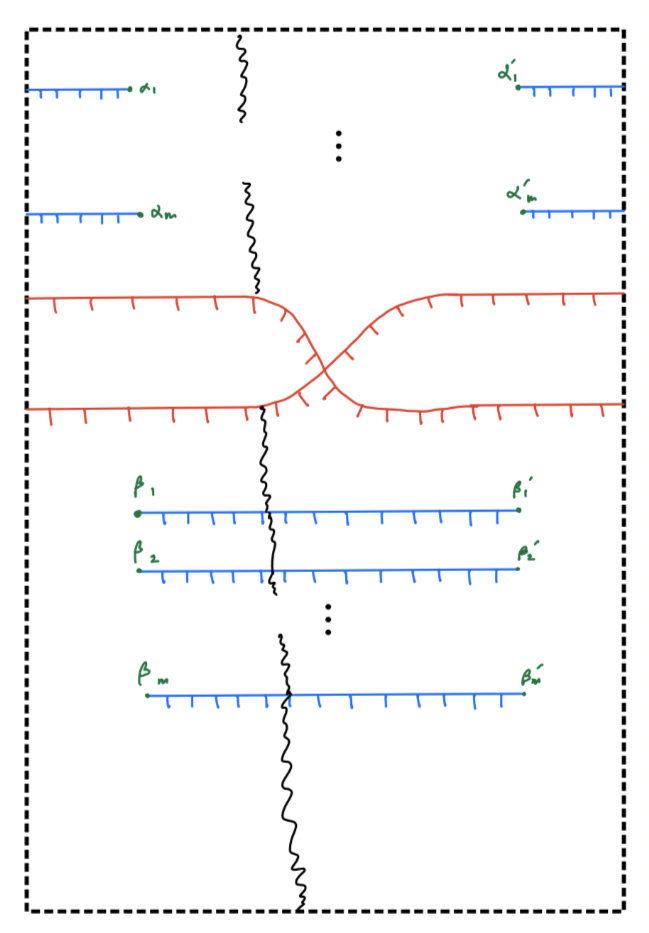
\includegraphics[scale=0.95]{diagrams/lemma11/2.png} % Adjust the width as needed
    \caption{Your caption here}
    \label{fig:your-label}
\end{figure}
In the above diagram I have intentionally omitted lines connecting \\
- $\alpha_i$ and $\beta_i$ for $i=1,\cdots ,m$\\
- $\alpha'_i$ and $\beta'_i$ for $i=1,\cdots ,m$\\

so as not to make diagram too messy. These omitted lines are mutually disjoint and crosses each red strand at most once. \\

Let the crossing of $\overline{\alpha_j \beta_j}$ with the upper(lower resp.) red strand be called $c_{0,j}$($c_{1,j}$ resp.) and $\overline{\alpha'_j \beta'_j}$ be called $c;_{0,j}$($c'_{1,j}$ resp.)\\

Let's denote the north, east, west, south of the crossing $c_{i,j}$($c'_{i,j}$ resp.) as $N_{i,j},E_{i,j},W_{i,j},S_{i,j}$($N'_{i,j},E'_{i,j},W'_{i,j},S'_{i,j}$ resp.)\\

The final sheaf will be describe as follows:\\

Stalks :\\
- $E_{i,j}$ : $\mathbb{C}^{m+1+i-j}$\\
- $S_{i,j}$ : $\mathbb{C}^{m+i-j}$\\
- $W_{i,j}$ : $\mathbb{C}^{m+1+i-j}$\\
- $N_{i,j}$ : $\mathbb{C}^{m+2+i-j}$\\

- $E'_{i,j}$ : $\mathbb{C}^{m+1+i-j}$\\
- $S'_{i,j}$ : $\mathbb{C}^{m+i-j}$\\
- $W'_{i,j}$ : $\mathbb{C}^{m+1+i-j}$\\
- $N'_{i,j}$ : $\mathbb{C}^{m+2+i-j}$\\

Generization maps:\\
- maps crossing red strands are $\iota_f$ and maps crossing blue strands are $\iota_l$ unless mentioned otherwise\\
- So I will describe the maps crossing squiggly lines, non $\iota_f,\iota_l$ maps only.\\
\\
- $E_{1,j}\rightarrow W'_{1,j}$ : 
$
\begin{pmatrix}
		\begin{matrix} 
			d_{j+1} & \cdots & 0 \\ 
			\vdots & \ddots & \vdots\\
			0 & \cdots & d_m
		\end{matrix} & \vline &
		\begin{matrix}
			0&0\\
			\vdots&\vdots\\
			0&0
		\end{matrix}\\
		\hline
		\begin{matrix}
			0&\cdots&0\\
			0&\cdots&0
		\end{matrix}
		& \vline &
		\begin{matrix}
			a&0\\
			b& d
		\end{matrix}
\end{pmatrix}
$\\

- $W_{0,1}\rightarrow E'_{0,1}$ : $D_{1,m}$\\
\\
- $N_{1,1}\rightarrow N'_{1,1}$ : 
$
\begin{pmatrix}
		\begin{matrix} 
			d_{1} & \cdots & 0 \\ 
			\vdots & \ddots & \vdots\\
			0 & \cdots & d_m
		\end{matrix} & \vline &
		\begin{matrix}
			0&0\\
			\vdots&\vdots\\
			0&0
		\end{matrix}\\
		\hline
		\begin{matrix}
			0&\cdots&0\\
			0&\cdots&0
		\end{matrix}
		& \vline &
		\begin{matrix}
			a&0\\
			b& d
		\end{matrix}
\end{pmatrix}
$\\
\\
- $W_{1,1}\rightarrow W'_{1,1}$ : 
$
\begin{pmatrix}
		\begin{matrix} 
			d_{1} & \cdots & 0 \\ 
			\vdots & \ddots & \vdots\\
			0 & \cdots & d_m
		\end{matrix} & \vline &
		\begin{matrix}
			0\\
			\vdots\\
			0
		\end{matrix}\\
		\hline
		\begin{matrix}
			0&\cdots&0\\
			0&\cdots&0
		\end{matrix}
		& \vline &
		\begin{matrix}
			a\\
			b
		\end{matrix}
\end{pmatrix}
$\\
\\
- $E'_{0,1}\rightarrow E_{0,1}$ : 
$
\begin{pmatrix}
		\begin{matrix} 
			d_{1}^{-1} & \cdots & 0 \\ 
			\vdots & \ddots & \vdots\\
			0 & \cdots & d_m^{-1}
		\end{matrix} \\
		\hline
		\begin{matrix} 
			0 & \cdots & 0 
		\end{matrix} 
\end{pmatrix}
$\\

If $m=1$, $isotopy_{11}$ is just $isotopy_{10}$.\\
Suppose we have defined $isotopy_{11}$ upto the number of blue strands less than $m$. Let's define $isotopy_{11}$ for the number of blue strands equals $m$:\\

(step1) Apply $isotopy_11$ for the number of blue strands equals $m-1$ on the disk surrounded by purple dotted line which is well-defined by induction hypothesis

\begin{figure}[H] % Optional: [h] means here, [t] for top, [b] for bottom, [p] for page of floats
    \centering
    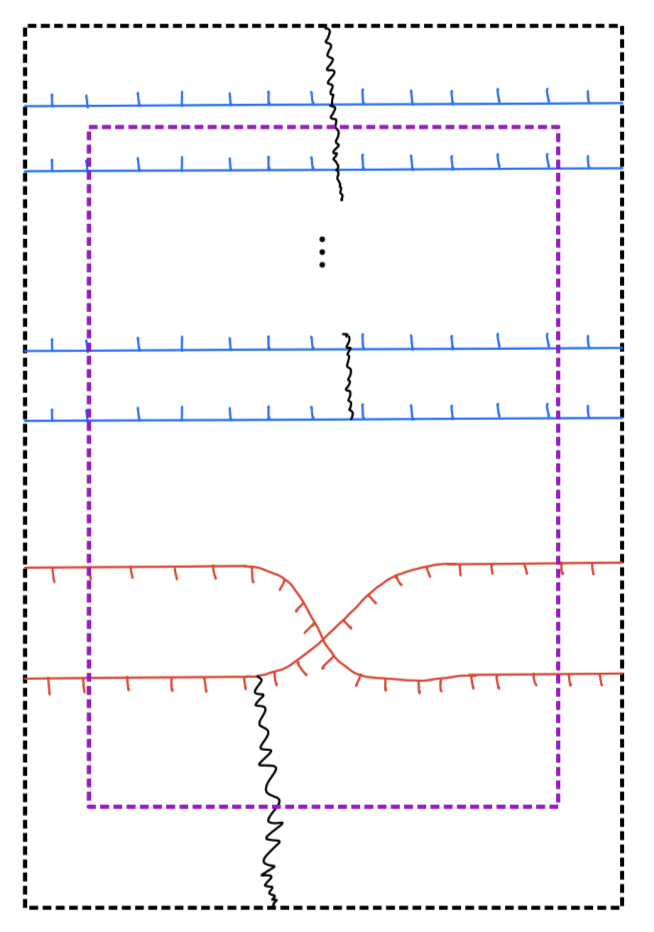
\includegraphics[scale=0.95]{diagrams/lemma11/3.png} % Adjust the width as needed
    \caption{Your caption here}
    \label{fig:your-label}
\end{figure}

We get the following diagram:

\begin{figure}[H] % Optional: [h] means here, [t] for top, [b] for bottom, [p] for page of floats
    \centering
    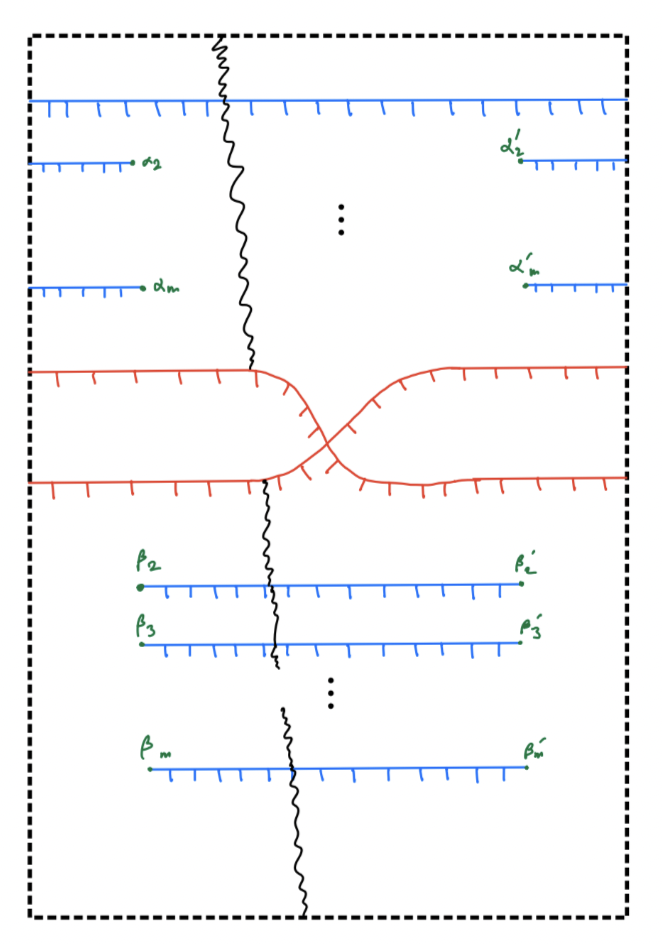
\includegraphics[scale=0.95]{diagrams/lemma11/4.png} % Adjust the width as needed
    \caption{Your caption here}
    \label{fig:your-label}
\end{figure}

(step2) Apply $isotopy_{10}$ on the disk surrounded by purple dotted line:

\begin{figure}[H] % Optional: [h] means here, [t] for top, [b] for bottom, [p] for page of floats
    \centering
    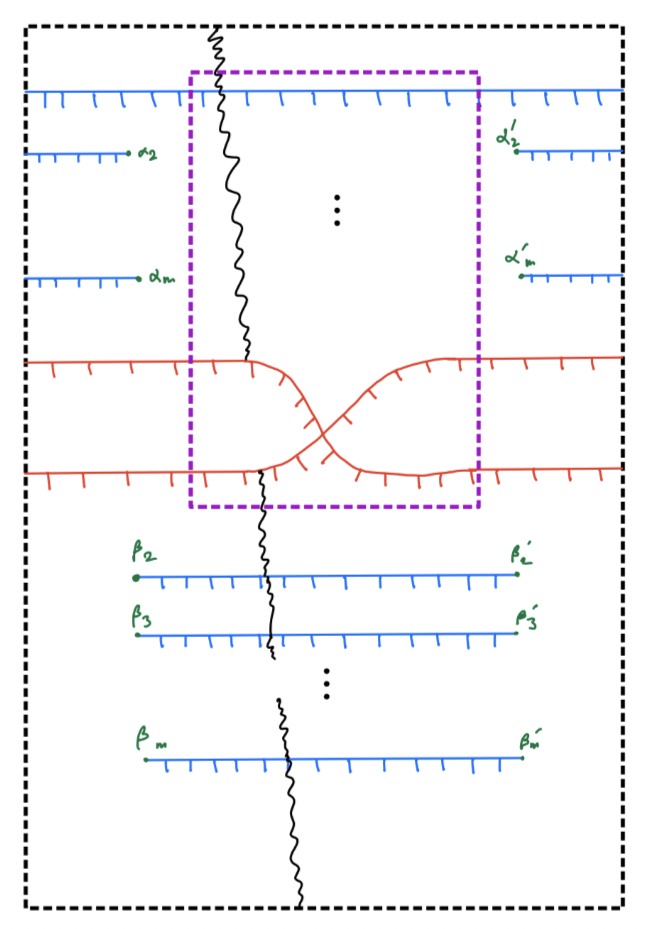
\includegraphics[scale=0.95]{diagrams/lemma11/5.png} % Adjust the width as needed
    \caption{Your caption here}
    \label{fig:your-label}
\end{figure}

We get the final diagram:

\begin{figure}[H] % Optional: [h] means here, [t] for top, [b] for bottom, [p] for page of floats
    \centering
    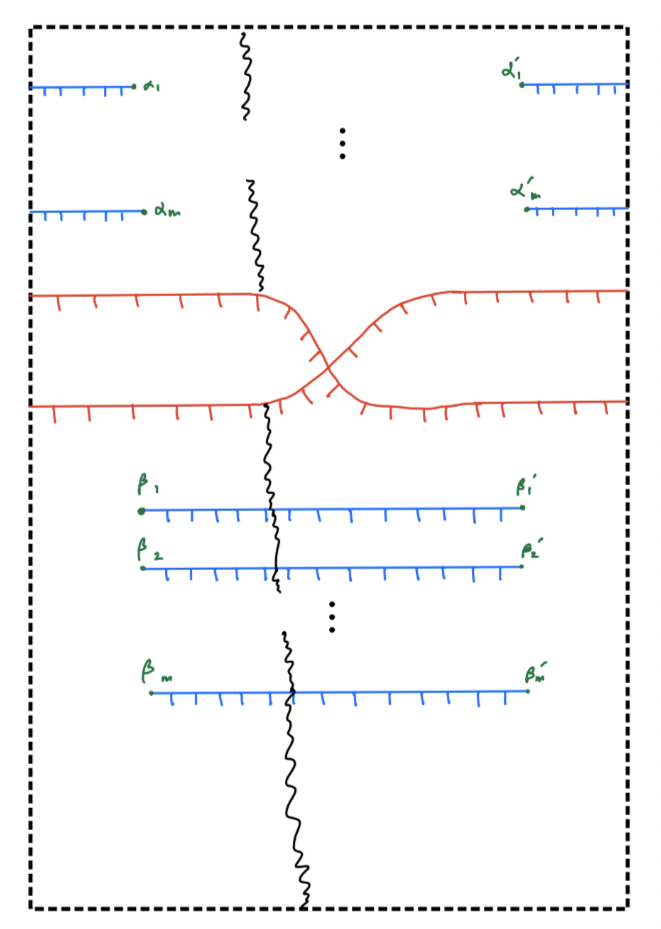
\includegraphics[scale=0.95]{diagrams/lemma11/6.png} % Adjust the width as needed
    \caption{Your caption here}
    \label{fig:your-label}
\end{figure}

with $\mathfrak{F}'$ on it.\\
(proof)